\hypertarget{appendix-8a046b38375e}{}
\section*{Phase 5 - Algorithms by Workload - Visual Recall}
\section{An asset request becomes a data structure, graph and scheduling decision}\label{appendix-8a046b38375e-an-asset-request-becomes-a-data-structure-graph-and-scheduling-decision}

This companion tests independent reconstruction, not recognition of terminology. The full, concept-led teaching runs from \hyperref[01-foundations-i-ch007-the-scene-is-now-too-large-for-the-wrong-container-phase-5-m025m027-parts-401445]{the asset data model} to \hyperref[01-foundations-i-ch008-from-an-asset-map-to-a-correct-navigable-world-phase-5-m028m030-parts-446500]{navigation, sorting, scans and caches}. All exact original parts and which of them have executable evidence are in \hyperref[appendix-fd090d982a15-phase-5-algorithms-and-data-structure-workload-contracts-parts-401500]{the contract ledger}. The test reference is \hyperref[source-file-0ec69e1a1a11439bca29faa5]{the standalone C++20 lab}.

\subsection{The first decision: what is the abstract promise?}\label{appendix-8a046b38375e-the-first-decision-what-is-the-abstract-promise}

The editor must look up a mesh name, enumerate assets in sorted order, update component storage, process streaming requests and repeatedly find the next shortest tentative route. Describe the operations and required ordering separately, then choose a concrete representation. Explain why a map, ordered map, vector, ring, priority queue and sparse set are \emph{different answers} even when they all store references to the same assets. Derive a Big-O bound using an explicit input size and constants, then explain why this bound does not predict cache-miss or allocator cost.

\textbf{Answer to verify against:} A workload chooses an ADT first, and that ADT defines operations. Different representations implement the ADT with different time, space, invalidation and ordering properties. Expected hashing cost requires a distribution/quality assumption; tree worst-case cost requires a balancing invariant. The Phase 4 hardware model supplies the missing locality and bandwidth dimensions.

\subsection{Dynamic storage and wraparound}\label{appendix-8a046b38375e-dynamic-storage-and-wraparound}

Derive the geometric series showing that vector's O(n) occasional relocation leads to O(1) \emph{amortized} append across n appends under geometric capacity growth. Explain why the worst-case \emph{one} append remains O(n), and which iterators or pointers reallocation invalidates. Then implement a fixed-capacity ring that distinguishes full from empty without one permanently unused slot. Trace: push 10,20,30; reject 40; pop 10,20; push 40,50; pop 30,40,50. State where object lifetimes begin and end when ring slots contain nontrivial types.

\textbf{Answer to verify against:} Store head and count, with tail=(head+count) mod C and 0≤count≤C. The lab uses optional slot values; this is a single-thread FIFO, not a correct multi-producer lock-free ring. A deque or linked list offers different mutation/iterator contracts.

\subsection{A hash collision is an algorithm, not a rare exception}\label{appendix-8a046b38375e-a-hash-collision-is-an-algorithm-not-a-rare-exception}

Draw a table where keys 1,9,17 collide under modulo-eight indexing. Place entries using linear probing, delete one in the middle, then show why an unoccupied tombstone cannot terminate a later lookup. Design insertion that remembers a tombstone but still searches for a duplicate key farther along the chain. Distinguish linear probing, quadratic probing, Robin Hood displacement, separate chaining and immutable perfect hashing; explain when each requires rehashing or special deletion rules.

\textbf{Answer to verify against:} A never-used slot terminates a probe chain; a tombstone does not. The lab includes growth and 1,200 reproducible mutations compared to std::unordered\_map. It does not claim Robin Hood or perfect hashing is implemented. Expected constant-time performance is conditional.

\subsection{A probabilistic structure makes a one-sided claim}\label{appendix-8a046b38375e-a-probabilistic-structure-makes-a-one-sided-claim}

Derive the Bloom filter approximate false-positive probability (1−e\textsuperscript{(−kn/m))}k and state the independence/uniformity assumption. A query whose kth bit is zero proves absence under a no-deletion contract; all-one bits permit a false positive. Explain why clearing a shared bit on deletion can create a false negative for another inserted key. Compare Bloom membership with exact bitsets and exact hashed sets.

\textbf{Answer to verify against:} Never assert that Bloom query positives prove membership. The lab only asserts no false negatives for known inserted keys.

\subsection{Tree invariants and heaps}\label{appendix-8a046b38375e-tree-invariants-and-heaps}

Explain why an unbalanced BST can degenerate from O(log n) to O(n), and reconstruct one AVL rotation preserving in-order traversal. State the red-black invariants that bound tree height. Compare a B-tree and B+ tree in terms of block/page accesses and range scans. Now trace binary-heap insertion into an array, list its parent and child indices and show why the heap property is weaker than global sorted order. Explain why a priority queue supports Dijkstra even if it allows stale entries.

\textbf{Answer to verify against:} AVL/red-black/B+/radix implementations are not in the current lab; independent adversarial insertion/deletion oracles are still required. The lab uses a standard-library heap to test actual graph distances.

\subsection{From graph meaning to valid paths}\label{appendix-8a046b38375e-from-graph-meaning-to-valid-paths}

Construct one directed four-vertex graph with weights 0→1=2, 0→2=5, 1→2=1, 1→3=10 and 2→3=1. Trace BFS hops, Dijkstra distances, Bellman--Ford relaxations, A* g/h/f values and Floyd--Warshall D\_k updates. Explain why BFS returns hop counts {[}0,1,1,2{]} while Dijkstra returns {[}0,2,3,4{]}. Add a negative edge and show why Dijkstra's greedy proof fails. Then create a reachable negative cycle and show how one extra Bellman--Ford relaxation detects it.

\textbf{Answer to verify against:} Nonnegative weights are essential for Dijkstra's usual correctness argument; A* requires an admissible heuristic for optimality under the stated algorithm/termination rules, and consistency provides an additional edgewise inequality. The lab's A* does not certify a caller-supplied heuristic. Floyd--Warshall is an independent O(V³) oracle on bounded small graphs, not necessarily the best production navigator.

\subsection{Directed dependencies and undirected connectivity}\label{appendix-8a046b38375e-directed-dependencies-and-undirected-connectivity}

Draw a pass DAG. Compute indegrees and perform Kahn's topological sort. Add an edge from the final node to the first and explain why no topological order can exist. Then describe SCC condensation and why cycles require an explicit feedback/error policy rather than a lucky traversal order. For an undirected weighted graph, trace Kruskal's sorted edges and DSU unions and justify the selected edge using the cut property. Compare to Prim without mistaking an MST for shortest paths.

\textbf{Answer to verify against:} The graph lab detects cycles, computes an MST of cost six and tests DSU unions. It does not implement all SCC and Prim variants; those require additional implementation witnesses.

\subsection{When integer order becomes a buffer-offset proof}\label{appendix-8a046b38375e-when-integer-order-becomes-a-buffer-offset-proof}

From counts {[}3,0,4,2{]}, derive the exclusive scan {[}0,3,3,7{]} and total nine; list each half-open output interval and prove they cannot overlap. Contrast inclusive {[}3,3,7,9{]}. Show the overflow condition for a 64-bit unsigned total. Explain why a GPU parallel scan requires group-level communication and additional global coordination, whereas a serial CPU scan needs only one sequential accumulator. Explain Morton key interleaving for coordinates (1,2), yielding nine, and give an example of why Z-order is not globally sorted Euclidean distance.

\subsection{Sorting needs an input and comparator contract}\label{appendix-8a046b38375e-sorting-needs-an-input-and-comparator-contract}

Compare insertion, selection, bubble, merge, quick, heap, introsort, counting and radix sorting. Include worst-case complexity, memory, stability and suitability for nearly sorted input or small integer keys. Explain why binary and lower-bound search cannot be run on an unsorted range and why NaN comparison without a total-order policy can violate the comparator contract. Give one workload where stable sorting is required and one where ordered iteration is irrelevant.

\subsection{Dynamic programming, randomized selection and caches}\label{appendix-8a046b38375e-dynamic-programming-randomized-selection-and-caches}

Show why choosing the largest denomination first fails for \{1,3,4\} and target six, and derive the DP recurrence for the minimum number of coins. Explain when memoization and tabulation produce identical answers but different execution/storage patterns. Prove one-element reservoir sampling uniform by induction; distinguish a fixed random seed from an unbiased generator. Explain the Fisher--Yates swap range. Build an LRU cache from a list plus hash index, trace its eviction at capacity two, then connect stable handles to sparse-set swap-removal and generation checking.

\subsection{The final performance decision}\label{appendix-8a046b38375e-the-final-performance-decision}

Given the same asset count and query/update workload, compare an open-addressed table, balanced tree, sorted vector, sparse set and direct-index table. Record correctness invariants and whether iteration pointers survive mutation. Design benchmark distributions over n, hash collisions, hit/miss ratios, entity churn, graph density and memory pressure. Profile before naming a winner. An example-only test is not evidence of expected-case performance for arbitrary production input.

\textbf{Independent mastery gate:} reproduce a FIFO, tombstone probe, heap priority rule, Dijkstra relaxation, topological Kahn step, DSU union and exclusive scan without looking up the source; then explain exactly what breaks when the preconditions fail. The source-to-claim chain should remain inspectable, and no current Kairo code is claimed verified unless actually read.

\subsection{Recall the recursive cost before naming its theorem}\label{appendix-8a046b38375e-recall-the-recursive-cost-before-naming-its-theorem}

\pandocbounded{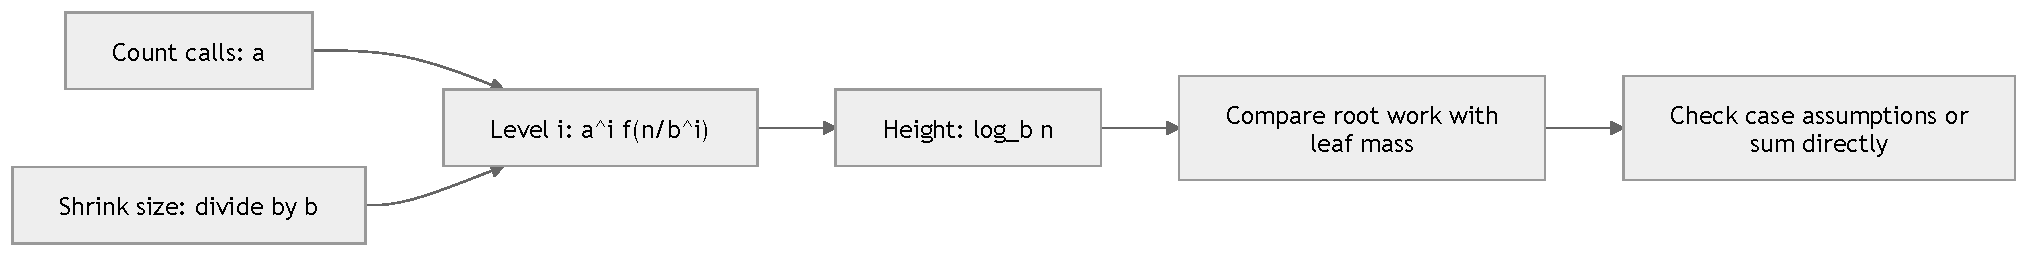
\includegraphics[keepaspectratio,alt={Diagram}]{../Assets/Print/303e95c801478a962025ae09fd03b1bf3d4a5b6118301749c83503f4f6d5ddda.pdf}}

{\def\LTcaptype{none} % do not increment counter
\begin{longtable}[]{@{}
  >{\raggedright\arraybackslash}p{(\linewidth - 4\tabcolsep) * \real{0.3333}}
  >{\raggedright\arraybackslash}p{(\linewidth - 4\tabcolsep) * \real{0.3333}}
  >{\raggedright\arraybackslash}p{(\linewidth - 4\tabcolsep) * \real{0.3333}}@{}}
\toprule\noalign{}
\begin{minipage}[b]{\linewidth}\raggedright
Recall prompt
\end{minipage} & \begin{minipage}[b]{\linewidth}\raggedright
Short answer
\end{minipage} & \begin{minipage}[b]{\linewidth}\raggedright
Return to the teaching
\end{minipage} \\
\midrule\noalign{}
\endhead
\bottomrule\noalign{}
\endlastfoot
What must a recurrence include? & Recursive-call costs, work outside the calls, and a base cost. & {[}{[}Continuous Notes/Computing Foundations - From Bits to C++ and Systems APIs\#A recurrence turns recursive calls into a cost equation \\
Why does mergesort gain a logarithm? & Each of \(\log_2 n\) non-leaf levels costs \(n\); leaves add \(n\). With \(T(1)=1\), \(T(8)=32\). & {[}{[}Continuous Notes/Computing Foundations - From Bits to C++ and Systems APIs\#A recurrence turns recursive calls into a cost equation \\
Can every smaller-than-\(n\) term use Case 1? & No.~\(n/\log n\) is not polynomially smaller. Its tree gives \(\Theta(n\log\log n)\). & {[}{[}Continuous Notes/Computing Foundations - From Bits to C++ and Systems APIs\#A recurrence turns recursive calls into a cost equation \\
What is the extra Case 3 check? & For some \(c<1\), \(a f(n/b)\le c f(n)\) eventually. & {[}{[}Continuous Notes/Computing Foundations - From Bits to C++ and Systems APIs\#A recurrence turns recursive calls into a cost equation \\
\end{longtable}
}
